%------------------------------------------------------------------------
\begin{frame}
	\frametitle{Aufgabe 2) Gradient}
	\framesubtitle{Aufgabenbeschreibung}
	\setbeamertemplate{enumerate items}[default]
	Gegeben:
	\begin{flalign*}
		a,b,Z,L,J,Y,m,n,s, \Delta Z
	\end{flalign*}
	Gesucht:
	\begin{flalign*}
		\gamma, \Gamma
	\end{flalign*}
	Wobei:
	\begin{flalign*}
		\gamma &= b + Y \Sigma(I-L\Sigma)^{-1} a \\
		\Gamma &= J + Y \Sigma(I-L\Sigma)^{-1} Z
	\end{flalign*}
	\begin{flalign*}
		\Sigma = Diag(Sign(\Delta z))
	\end{flalign*}
	\begin{flalign*}
	\begin{pmatrix}
	\Delta z \\
	\Delta y
	\end{pmatrix}
	= 
	\begin{pmatrix}
	a \\
	b
	\end{pmatrix}
	+
	\begin{pmatrix}
	Z & L \\
	J & Y 
	\end{pmatrix}
	\times
	\begin{pmatrix}
	\Delta x \\
	|\Delta z |
	\end{pmatrix}
	\end{flalign*}
	
\end{frame}
%------------------------------------------------------------------------
\begin{frame}
	\frametitle{Aufgabe 2) Gradient}
	\framesubtitle{Interssanter Teil}
	\setbeamertemplate{enumerate items}[default]
	Brauchen:
	\begin{flalign*}
		\Sigma(I-L\Sigma)^{-1}
	\end{flalign*}
	\begin{flalign*}
		\Sigma = Diag(Sign(\Delta z))
	\end{flalign*}
	Fallstricken:
	\begin{itemize}
		\item Sparse Matrix $\Sigma$
		\item Inverse $(I-L\Sigma)^{-1}$
	\end{itemize}
	
\end{frame}
%------------------------------------------------------------------------
\begin{frame}
	\frametitle{Aufgabe 2) Gradient}
	\framesubtitle{Beispiel}
	\setbeamertemplate{enumerate items}[default]
	
	Sei:
	\begin{flalign*}
		\Delta z = [-3, 0, 4,  -1]
	\end{flalign*}
	Dann gilt für $I - L\Sigma$:
	\begin{flalign*} 
	I -
	\left(\begin{array}{cccc}
	0 		& 0 	  & 0  & 0 \\
	L_{2,1} & 0 	  & 0  & 0 \\
	L_{3,1} & L_{3,2} & 0  & 0\\
	L_{4,1} & L_{4,2} & L_{4,3} & 0 \\
	\end{array}\right) \times
	\left(\begin{array}{cccc}
	-1 & 0 & 0 & 0 \\
	0 & 0 & 0 & 0 \\
	0 & 0 & 1 & 0 \\
	0 & 0 & 0 & -1 \\
	\end{array}\right)
	= 
	\left(\begin{array}{cccc}
	1 & 0 & 0 & 0 \\
	-L_{2,1} & 1 & 0 & 0 \\
	-L_{3,1} & 0 & 1 & 0 \\
	-L_{4,1} & 0 & 0 & 1 \\
	\end{array}\right)
	\end{flalign*}
	das entspricht folgenden Operationen:
	\begin{itemize}
		\item Hinzufügen einer Hauptdiagonalen
		\item Skalieren der Spalten von $L$ mit den Vorzeichen von $\Delta z$
	\end{itemize}
	Besser dieses als Operation zu implementieren.
	Das Auflösen der unteren Dreiecksmatrix $(I-L\Sigma)^{-1}$ übernimmt CUBLAS.
\end{frame}
%----------------------------------------------------------------------------
\begin{frame}[fragile]
	\frametitle{Aufgabe 1) Gradient}
	\framesubtitle{Implementierung}
	\begin{lstlisting}[language=cpp]
	template <typename T>
	void gradient(T *a, T *b, 
				  T *Z, T *L, 
				  T *J, T *Y,
				  T *dz,
				  T *Tss, T *I, T *K,
				  int m, int n, int s,
				  int gridsize, int blocksize,
				  T *gamma, T *Gamma)
		//  d_Tss = diag(1) - L * diag(sign(dz))
		initTss <<<gridsize, blocksize >>>(d_Tss,d_L, d_dz, s, s*s);
		//  d_I = diag(1) // room for improvement, operations can be merged		
		initIdentity <<<gridsize, blocksize >>> (d_I, s);
		//  d_I = d_Tss * X	
		getTriangularInverse(handle, d_Tss, d_I, s);
		//	d_I = d_I * diag(sign(dz))
		multWithDz <<<gridsize, blocksize >>>(d_I, d_dz, s);
		//	d_K = d_Y * d_I
		cublasDgemm(.,d_Y,.,d_I,d_K,));
		//	d_gamma = d_b
		//  d_Gamma = J
		cudaMemcpy(d_gamma, d_b,.);
		cudaMemcpy(d_Gamma, d_J,.);
		//	d_gamma = d_gamma + K*a
		cublasDgemv(.,d_K,., d_a,., d_gamma,.);
		//  d_Gamma = d_Gamma + K*Z
		cublasDgemm(.,d_K,d_Z,d_Gamma,m));
	}
	\end{lstlisting}
\end{frame}
%------------------------------------------------------------------------

\begin{frame}
	\frametitle{Aufgabe 2) Gradient}
	\framesubtitle{Speicherkomplexität}
	Speicherkomplexität: \\
	\begin{center}
		\begin{tabular}{ c | c | c | c | c | c | c | c | c | c | c | c }
			$a$ & $b$ & $Z$ & $L$ & $J$ & $Y$ & $\Delta z$ & $\gamma$ & $\Gamma$ & $Tss$ & $I$ & $K$\\
			\hline
			$s$ & $m$ & $s*n$ & $s*s$ & $m*n$ & $m*s$ & $s$ & $m$ & $m*n$& $s*s$ & $s*s$ & $m*s$\\
		\end{tabular}
	\end{center}
	Bei $m=n=s$:
	\begin{flalign*}
		8s^2 + 4s \times sizeof(type)
	\end{flalign*}
	\begin{itemize}
		\item $m=n=s=1000:$  0.064 GB
		\item $m=n=s=5000:$ 1.6 GB
		\item $m=n=s=10.000:$ 6.40 GB
	\end{itemize}
\end{frame}
%------------------------------------------------------------------------
\begin{frame}
	\frametitle{Aufgabe 2) Gradient}
	\framesubtitle{Komplexität}
	Komplexität $(m=n=s)$: \\
	\begin{center}
		\begin{tabular}{ l | l}
			Funktion & Komplexität Seriell \\
			\hline
			$initTss()$	& $s^2$\\
			$initIdentity()$& $s^2$ \\
			$getTriangularInverse()$& $s^2$ (backsubstitution)\\
			$multWithDz()$  & $s^2$  \\
			$cublasDgemm()$& $s^3$ \\
			$cublasDgemv()$ & $s^2$ \\
			$cudaMemcpy()$ & $s$ \\
		\end{tabular} 	\\~\\
	\end{center}
	Lässt sich alles gut parallel ausführen !!!
\end{frame}
\setbeamertemplate{navigation symbols}{}
\begin{frame}[plain]
	\makebox[\linewidth]{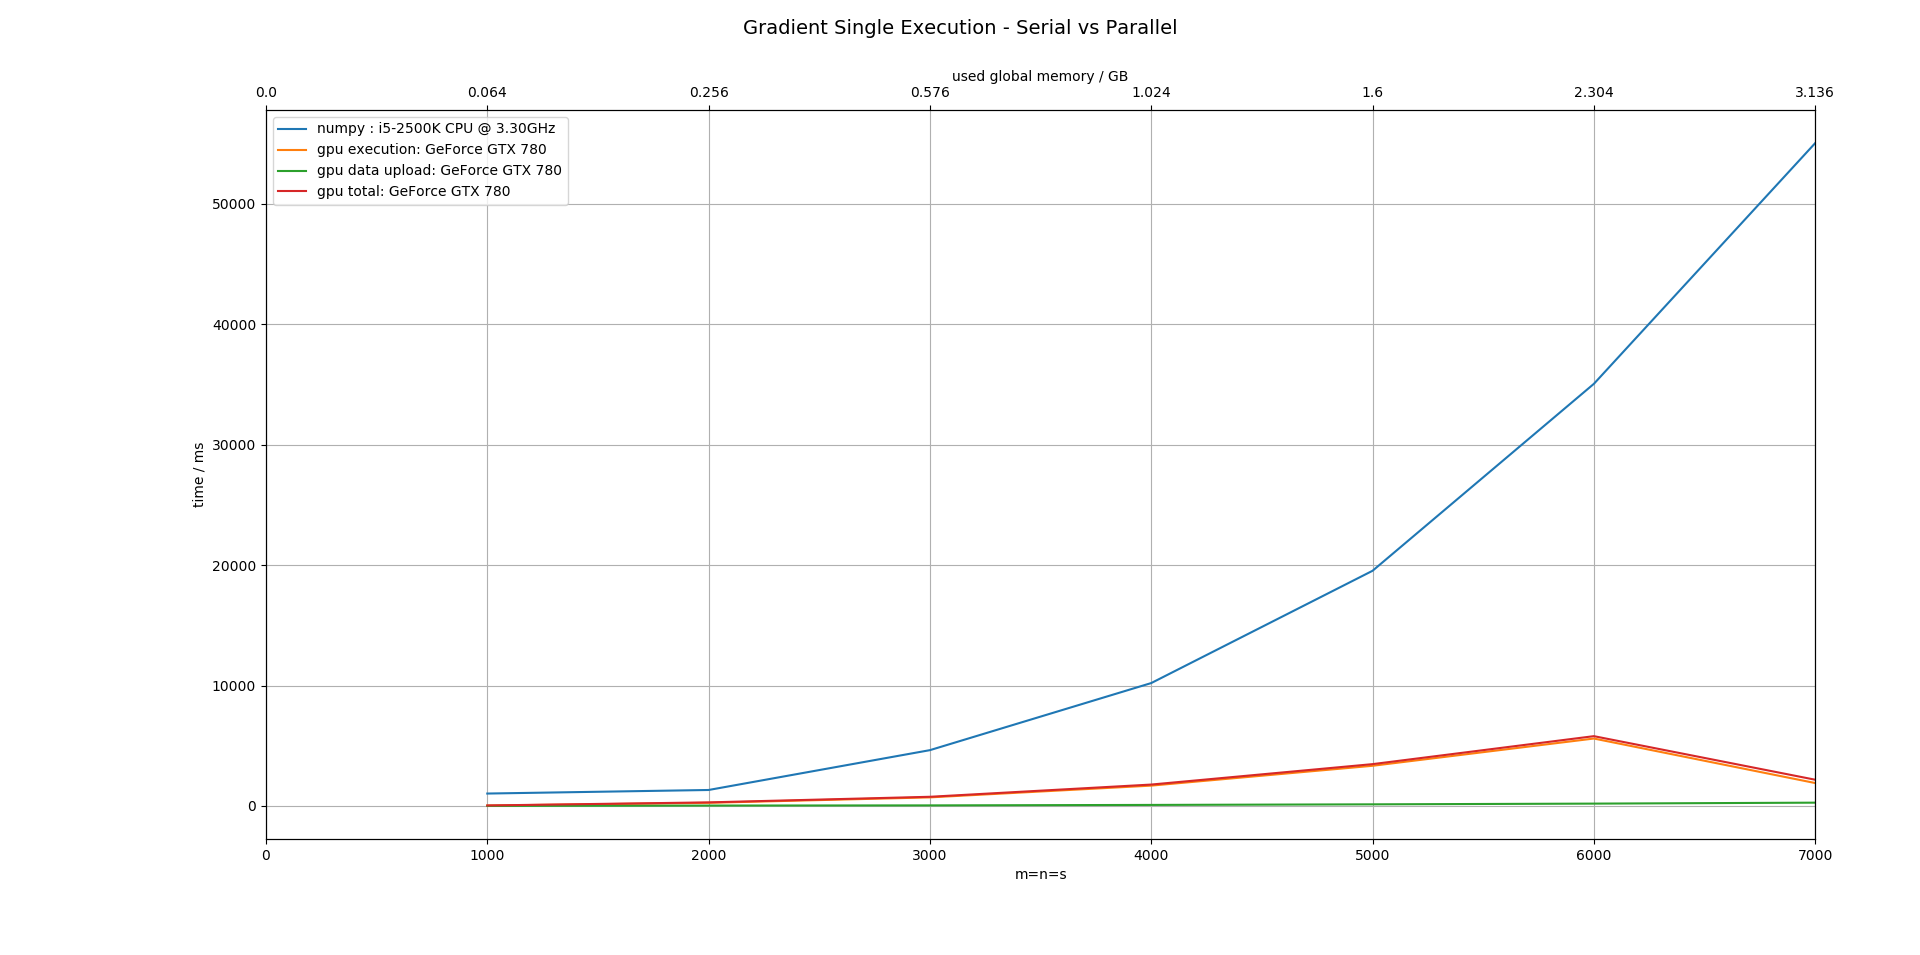
\includegraphics[width=\paperwidth]{img/grad-single.png}}
\end{frame}
%------------------------------------------------------------------------
\setbeamertemplate{navigation symbols}{}
\begin{frame}[plain]
	\makebox[\linewidth]{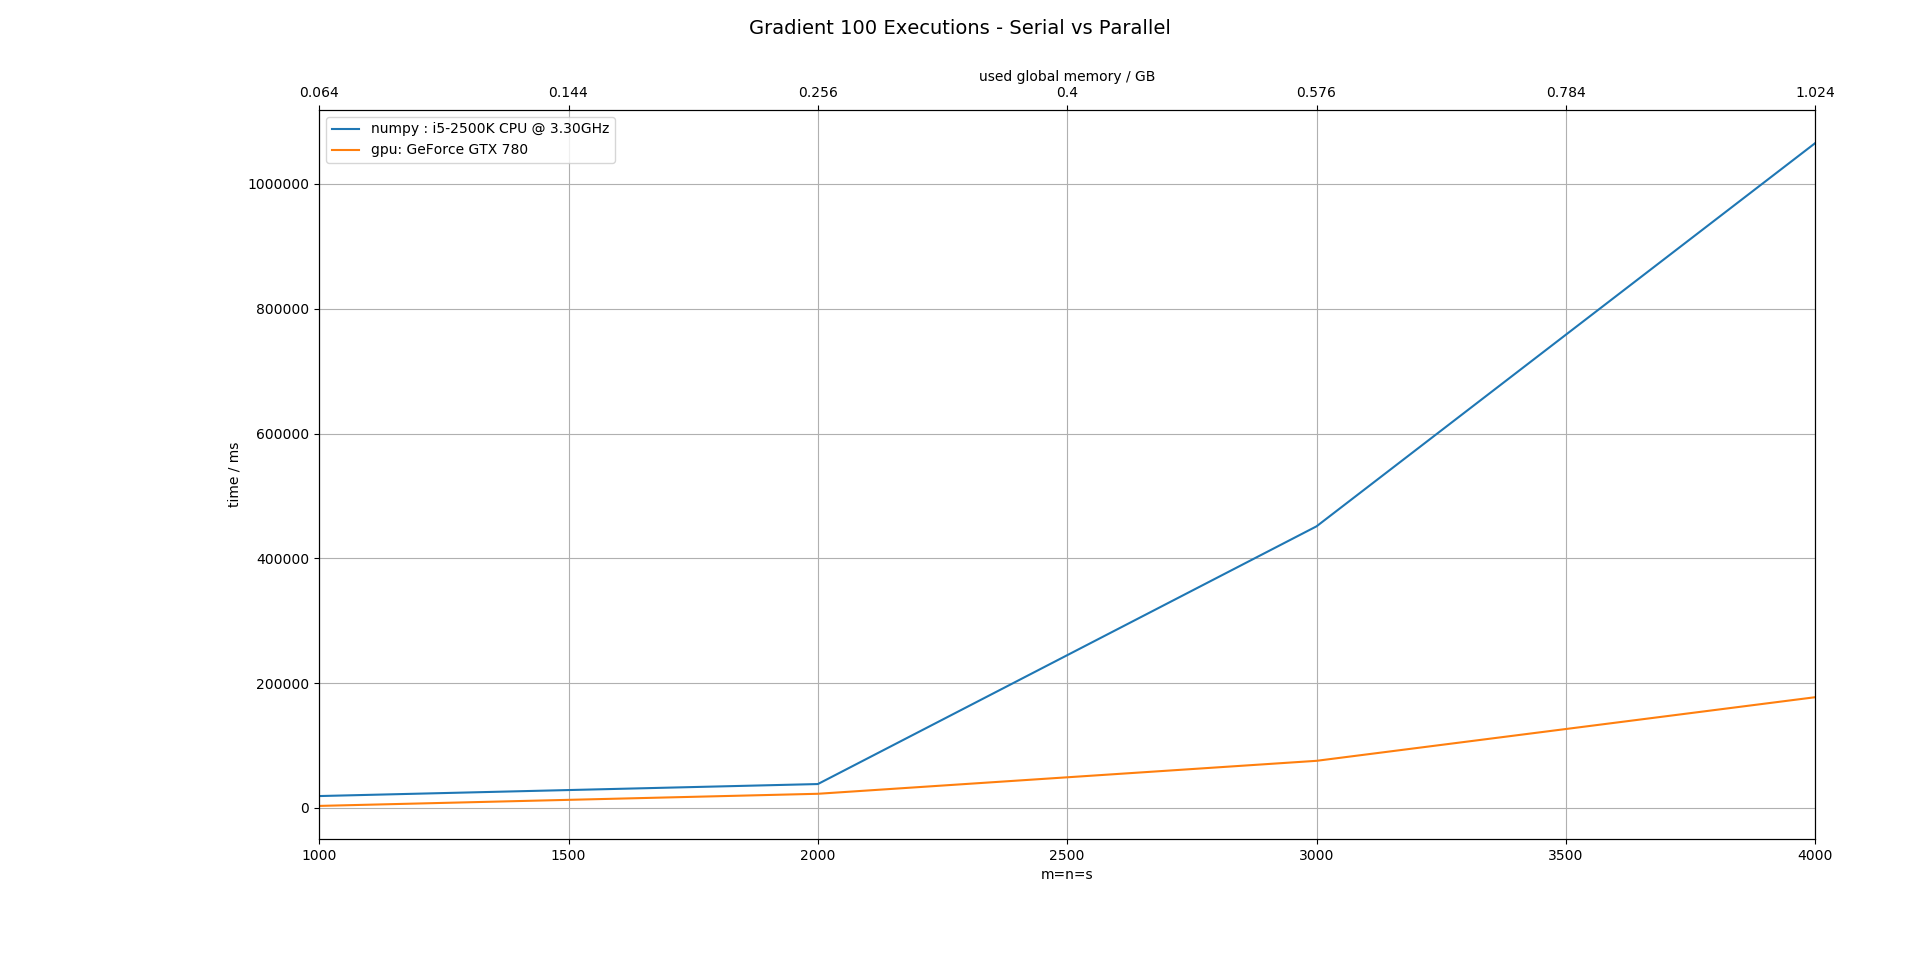
\includegraphics[width=\paperwidth]{img/grad-100.png}}
\end{frame}
%------------------------------------------------------------------------
\begin{frame}
	\frametitle{Aufgabenbeschreibung}
	\framesubtitle{Aufgabenbeschreibung - Solve}
	\setbeamertemplate{enumerate items}[default]
	
	\begin{flalign*}
	\left(\begin{array}{cccc}
	\tikzmarkin[ver=style cyan]{col 1}\x  & \x  & \tikzmarkin[ver=style green]{col 2} \x & \x \\
	0   & \x  & \x & \x \\
	0   & 0   & \x & \x \\
	0   & 0   & 0  & \x \\
	a \tikzmarkend{col 1}  &  b  &  c  \tikzmarkend{col 2} &  d \\
	\end{array}\right)
	\end{flalign*}
	\begin{flalign*}
	\begin{pmatrix}
	\Delta z \\
	\Delta y
	\end{pmatrix}
	= 
	\begin{pmatrix}
	a \\
	b
	\end{pmatrix}
	+
	\begin{pmatrix}
	Z & L \\
	J & Y 
	\end{pmatrix}
	\times
	\begin{pmatrix}
	\Delta x \\
	|\Delta z |
	\end{pmatrix}
	\end{flalign*}
	\begin{flalign*}
	\left(\begin{array}{c}
	\Delta z_1 \\
	\vdots \\
	\Delta z_s \\
	\Delta y_1 \\
	\vdots \\
	\Delta y_m
	\end{array}\right)  =
	\left(\begin{array}{c}
	a_1 \\
	\vdots \\
	a_s \\
	b_1 \\
	\vdots \\
	b_m \\
	\end{array}\right) +
	\left(\begin{array}{cccccc}
	Z_{1,1} & \dots & Z_{1,n} & 0 & \dots  & 0 \\
	\vdots & \ddots & \vdots  & L_x & \ddots & 0 \\
	Z_{s,1} & \dots & Z_{s,n} & L_x & L_x & 0 \\
	J_{1,1} & \dots & J_{1,n} & Y_{1,1} & \dots & Y_{1,s} \\
	\vdots  & \ddots & \vdots & \vdots & \ddots & \vdots \\
	J_{m,1} & \dots  & J_{m,n} & Y_{m,1} & \dots & Y_{m,s} \\
	\end{array}\right) \times
	\left(\begin{array}{c}
	\Delta x_1 \\
	\vdots \\
	\Delta x_n \\
	|\Delta z_1 | \\
	\vdots \\
	| \Delta z_s| \\
	\end{array}\right)
	\end{flalign*}
	
\end{frame}
%------------------------------------------------------------------------
\begin{frame}
\frametitle{Implementierung}
\framesubtitle{Client Side Storage}
	 BLOCKSIZE, GRIDSIZE OPTIMIZATION \\
	 ROW FORMAT, COL FORMAT \\
	 INTERFACE ??? \\
\end{frame}
%------------------------------------------------------------------------